\section{System Design}
\label{sec:system_design}

This chapter details the architectural design and implementation
strategies of the proposed \textit{PredCLOCK} system. The system is
designed as a hybrid simulation environment that bridges
high-performance cache simulation (written in C++) with predictive
machine learning models (trained in Python) to optimize cache
eviction decisions.

\subsection{System Architecture Overview}
The system architecture is constructed to ensure minimal latency
overhead while maintaining high prediction accuracy. As illustrated
in Figure~\ref{fig:system_architecture}, the system comprises three
main components: the Data Ingestion Layer (Trace Replay), the Core
Simulation Engine (LibCacheSim), and the Inference Engine (ONNX Runtime).

\begin{figure*}[t]
  \centering
  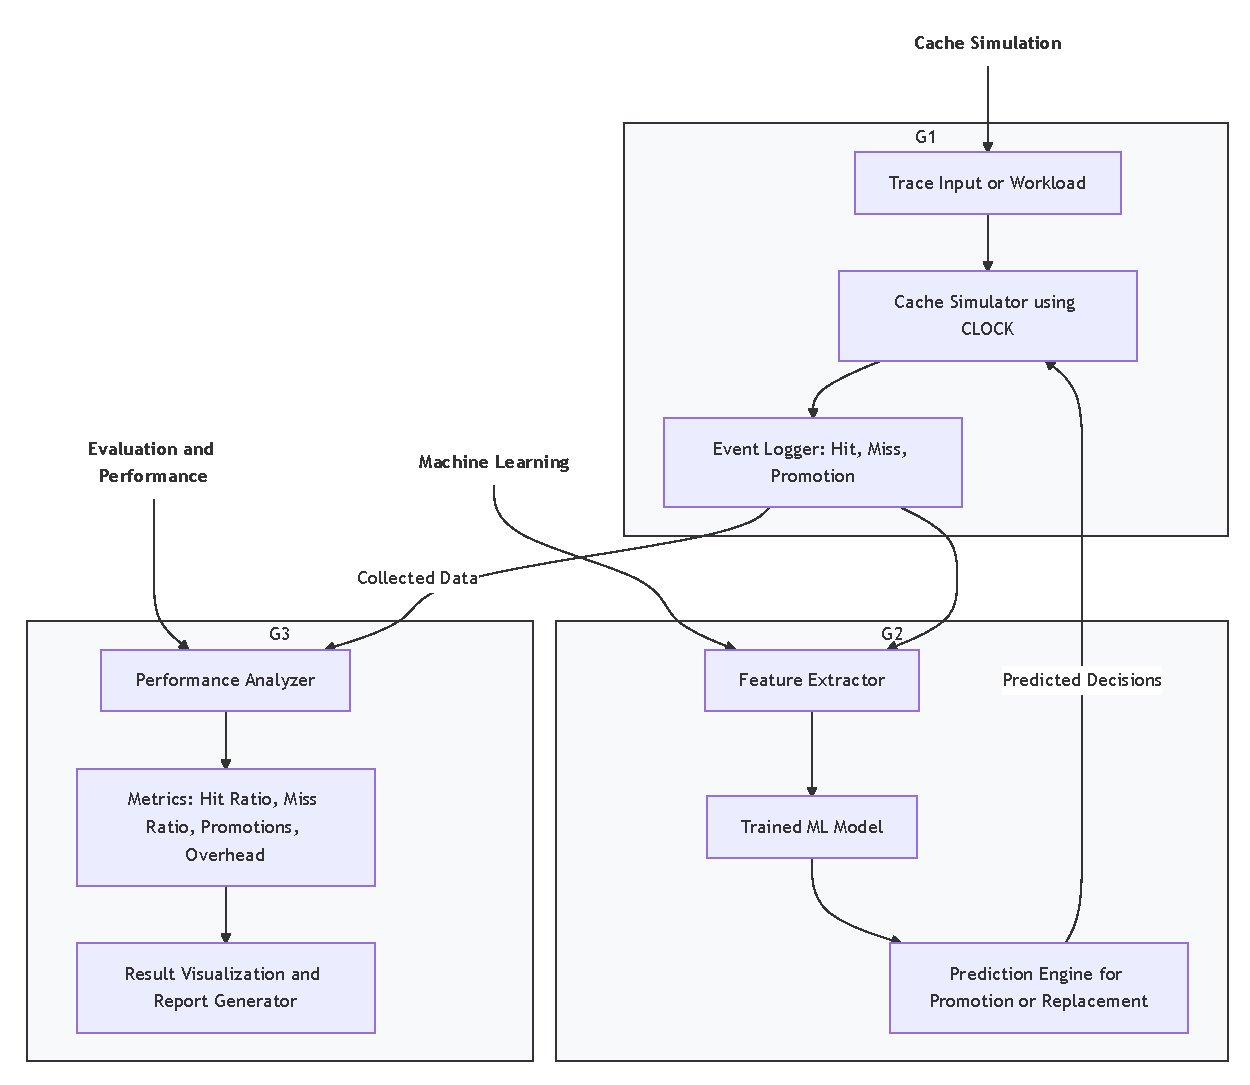
\includegraphics[width=1.0\linewidth]{figures/system-architecture.mmd.pdf}
  \caption{High-level system architecture showing the interaction
    between the Trace Replay mechanism, the Cache Simulator, and the ML
  Inference Engine via ONNX.}
  \label{fig:system_architecture}
\end{figure*}

The \textbf{Data Ingestion Layer} processes synthetic Zipfian traces
or real-world datasets, parsing object IDs and access timestamps.
These are fed into the \textbf{Core Simulation Engine}, which
implements the cache logic. Unlike standard CLOCK implementations,
our engine includes a hook to the \textbf{Inference Engine} whenever
a promotion decision is required. We utilize \textit{ONNX Runtime}
\cite{Tian2020Compiling} to execute the model within the C++
environment. This approach mitigates the interoperability costs and
latency overhead typically associated with Python-C++ context
switching during runtime \cite{Jajal2024Interoperability}.

\subsection{Program Workflow}
The research methodology follows a sequential workflow divided into
offline training and online inference phases.
Figure~\ref{fig:alur_program} outlines the complete flow of the program.

\begin{figure}[t]
  \centering
  
\includegraphics[width=0.8\linewidth]{figures/alur-program.mmd.pdf}
  \caption{Program workflow diagram illustrating the stages from
    Trace Generation, Labeling via Offline CLOCK, Model Training, to
  Final Simulation.}
  \label{fig:alur_program}
\end{figure}

The workflow consists of four distinct stages:
\begin{enumerate}
  \item \textbf{Trace Generation and Baseline Simulation:} Initial
    traces are run through a standard CLOCK simulator to establish
    baseline metrics such as hit ratio and eviction count.
  \item \textbf{Labeling (Offline Oracle):} We utilize an
    \textit{Offline CLOCK} algorithm with future knowledge to label
    dataset entries. Objects are labeled based on their utility:
    ``Wasted'' (promoted but never hit before eviction) or ``Reused''
    (promoted and subsequently hit) \cite{Zhang2025Rethinking}.
  \item \textbf{Training:} A lightweight neural network is trained
    using the labeled dataset to recognize patterns in frequency and recency.
  \item \textbf{Inference Integration:} The trained model is exported
    to the ONNX format and loaded into the modified simulator for the
    final evaluation.
\end{enumerate}

\subsection{Machine Learning Model Design}
The core of the decision-making process is a Supervised Learning
model designed to classify cache objects based on their likelihood of
future reuse.

\subsubsection{Model Architecture}
We employ a Multi-Layer Perceptron (MLP) defined using the Keras API
\cite{chollet2015keras}. As shown in Figure~\ref{fig:model_arch}, the
model takes a vector of features representing object history (e.g.,
frequency, reuse distance) and processes them through dense hidden
layers with ReLU activation.

\begin{figure*}[t]
  \centering
  
\includegraphics[width=0.6\linewidth]{figures/model-arch.mmd.pdf}
  \caption{Architecture of the Feed-Forward Neural Network used for
    eviction prediction. The final layer uses a Sigmoid activation to
  output a reuse probability score.}
  \label{fig:model_arch}
\end{figure*}

The output layer utilizes a \textit{Sigmoid} activation function,
producing a scalar probability score between 0 and 1. This score
represents the probability that promoting the object will result in a cache hit.

\subsubsection{Training Pipeline}
The training process, depicted in Figure~\ref{fig:ml_diagrams},
involves preprocessing raw trace logs into feature vectors. To
address class imbalance—where ``wasted'' promotions often outnumber
successful ones in specific workloads—we apply class weighting during
the training phase.

\begin{figure}[t]
  \centering
  
\includegraphics[width=0.5\linewidth]{figures/ml-diagrams.mmd.pdf}
  \caption{Machine Learning training pipeline, detailing feature
  extraction, data splitting, and model export to ONNX.}
  \label{fig:ml_diagrams}
\end{figure}

\subsection{Implementation and Decision Logic}
The integration of the model into the CLOCK algorithm alters the
standard eviction behavior to implement a ``Lazy Promotion'' strategy
\cite{chen2025lazy}. Figure~\ref{fig:model_impl} details the logic
flow during a cache eviction candidate check.

\begin{figure}[t]
  \centering
  
\includegraphics[width=0.8\linewidth]{figures/model-impl.mmd.pdf}
  \caption{Decision logic for the ML-Enhanced CLOCK Algorithm. The
    model acts as a filter for promotions, denying the ``second
  chance'' to low-utility objects.}
  \label{fig:model_impl}
\end{figure}

In a standard CLOCK algorithm, an object with a reference bit of 1 is
essentially guaranteed a ``second chance'' and remains in the cache.
In our PredCLOCK design, we intercept this process:
\begin{enumerate}
  \item When the clock hand points to an object with \texttt{ref\_bit
    = 1}, the system queries the ONNX model.
  \item If the model predicts a low probability of reuse ($P <
    Threshold$), the promotion is denied. The object is treated as if
    \texttt{ref\_bit = 0} and is evicted immediately.
  \item If the model predicts high reuse, the standard CLOCK logic
    proceeds: the reference bit is reset to 0, and the hand moves to
    the next candidate.
\end{enumerate}
This mechanism ensures that the cache is not polluted by
``one-hit-wonder'' objects that appear frequently in scan-heavy
workloads, addressing the specific weaknesses of CLOCK identified in
previous works \cite{Jiang2005CLOCKPro}.
